\section{The conditionally averaged Navier Stokes equations}
\label{ap:conditionally_navier_stokes}

In this appendix we revisit the method to derive the closure term of a stoke stain spherical droplets. 
Following \citet{zhang1994ensemble} we first demonstrate that in order to be closed the particle-averaged  fields need to be expressed in terms of \textit{single-particle} conditionally-averaged field. 
Then we demonstrate how to obtain these \textit{single-particle} conditionally-averaged field from what we call here the \textit{single-particle} conditionally-averaged equations. 

\subsection{The conditional average}
The first step is to introduce the relation between particle averaged field and \textit{single-particle} conditionally-averaged field.
For instance, let us take the example of the drag force term. 
Form the definition of the particle-average \ref{eq:p_avg} we write,
\begin{align}
    \pSavg{\bm\sigma_f^0\cdot\textbf{n}}[\textbf{x},t]
    &= \int \sum_{\alpha=1}^N \delta(\textbf{x}-\textbf{x}_\alpha[t; \FF])
    \int_{\Gamma_\alpha(t,\FF)}
    \bm\sigma_f^0\cdot\textbf{n}[\textbf{y},t;\FF]
    d\Gamma(\textbf{y}) d\PP
\end{align}
By writing this integral explicitly, we want to emphasize that the particle-averaged quantity is evaluated at the point \textbf{x}, while the integration over the surface of the particles $\alpha$ is carried out over the surface with the integration parameter $\textbf{y}$.
Therefore, we may enlarge the domain of integration from $\Gamma_\alpha$ to $\mathbb{R}^3$ by multiplying $\bm\sigma_f^0\cdot\textbf{n}(\textbf{r},t;\FF)$ with $\delta(|\textbf{y} - \textbf{x}_\alpha(t,\FF)| - a)$. 
It reads, 
\begin{equation}
    \pSavg{\bm\sigma_f^0\cdot\textbf{n}}[\textbf{x},t]
    = 
    \int_{\mathbb{R}^3}
    \int
     \sum_{\alpha=1}^N 
     \delta(\textbf{x}-\textbf{x}_\alpha(t; \FF))
    \delta(|\textbf{y} - \textbf{x}_{\alpha}(t;\FF)|-a)
    (\bm\sigma_f^0\cdot\textbf{n})[\textbf{y},t;\FF]
    d\PP
    d\textbf{y}
\end{equation}
Note that this definition is only valid for identical spherical particles of radius $a$. 
Due to the presence of $\delta(\textbf{x}-\textbf{x}_\alpha(t; \FF))$, this expression is non-zero only when $\textbf{x} = \textbf{x}_\alpha(\FF,t)$. 
Also, we can introduce the conditional average on the velocity of the particle by noticing that, 
\begin{equation*}
    \int_{\mathbb{R}^3} \delta(\textbf{c} - \textbf{u}_\alpha(\FF,t)) d\textbf{c} = 1. 
\end{equation*}
Taking in account the preceding remarks we are able to write
\begin{equation}
    \pSavg{\bm\sigma_f^0\cdot\textbf{n}}[\textbf{x},t]
    =
    n_p(\textbf{x})
    \int_{\mathbb{R}^3}
    \int_{|\textbf{x}-\textbf{y}|=a}
    \bm\sigma_f^1[\textbf{y},t;\textbf{x},\textbf{c}] \cdot \textbf{n}
    d\textbf{y}
    d\textbf{c}
    \label{eq:conditionally_averaged}
\end{equation}
where, 
\begin{equation*}
    \bm\sigma^1_f[\textbf{y},t;\textbf{x},\textbf{c}] n_p(\textbf{x},\textbf{c})
    =
    \avg{\delta_\alpha \bm\sigma^0_f}[\textbf{y},t;\textbf{x},\textbf{c}]
    = 
    \int 
    \sum_\alpha^N 
    \delta(\textbf{x} - \textbf{x}_\alpha(\FF,t))
    \delta(\textbf{c} - \textbf{u}_\alpha(\FF,t))
    \bm\sigma_f^0[\textbf{y},t;\FF]
    d\PP
\end{equation*}
is the \textit{single-particle} conditionally-averaged local stress of the continuous phase knowing that interface of the particle at $\textbf{x}$ is  present in \textbf{y}. 
In other world $\bm\sigma^1_f$ is the mean fluid phase stress evaluated at $\textbf{y}$ and time $t$ on every configuration where a particle is present at $\textbf{x}$. 
And $n_p(\textbf{x})$ is the number density but evaluated at $\textbf{x}$.
In light of \ref{eq:conditionally_averaged} we made the link between particle-average and the integral of a \textit{single-particle} conditionally-averaged quantity. 
Note that all quantities denoted with the superscript $^1$ refer to \textit{single-particle} conditionally-averaged  quantities.  
Therefore, it is implicit that these quantities are evaluated at $\textbf{y}$ and $t$ and conditionally on $\textbf{x}$. 

At some point it will also be useful to express continuous phase averaged quantities, i.e. $\avg{\chi_k f_k^0}$  in terms of one  \textit{single-particle} conditionally-averaged fields. 
Two examples are the Reynolds stress $\avg{\chi_f \textbf{u}_f'\textbf{u}_f'}$ and the fluid phase dissipation $\avg{\chi_f\sigma_f^0:\grad \textbf{u}_f^0}$ that appear in \ref{eq:dt_hybrid_rhou_f} and \ref{eq:dt_hybrid_k1}, respectively.  
To proceed one must first notice that, 
\begin{equation}
    \frac{1}{N}\sum_\alpha 
    \int_{\mathbb{R}^3}
    \int_{\mathbb{R}^3}
    \delta(\textbf{y}-\textbf{x}_\alpha)
    \delta(\textbf{c}-\textbf{u}_\alpha)
    d\textbf{x}
    d\textbf{c}
    = 1
\end{equation}
where $N$ is the total number of particle in the flow. 
Using this relation one may re-formulate the ensemble average of a continuous phase quantity as 
\begin{equation}
    \avg{\chi_k f_k^0}[\textbf{x},t]
    = 
    \frac{1}{N}
    \int_{\mathbb{R}^3}
    \int_{\mathbb{R}^3}
    f_k^1 P_1[\textbf{y},\textbf{c};\textbf{x},t] \phi_k[\textbf{x},t]
    d\textbf{y} 
    d\textbf{c}
    \label{eq:conditional_averaged_fluid}
\end{equation}
where,
\begin{equation*}
    f_k^1[\textbf{x},t;\textbf{y},\textbf{c}] P_1[\textbf{y},\textbf{c};\textbf{x},t] \phi_k[\textbf{x},t]
    =     
    \sum_i^N 
    \int
    \delta(\textbf{y}-\textbf{x}_i)
     \delta(\textbf{c}-\textbf{u}_i)
    \chi_k
    f^0_k[\textbf{x},t;\FF]
    d\PP.
\end{equation*}
In this expression $f_f^1[\textbf{x},t;\textbf{y},\textbf{c}]$ is the average of the local quantity $f_f^0$ evaluated at $\textbf{x}$ and time $t$ conditionally on the presence of a particle center of mass at $\textbf{y}$ with center of mass velocity $\textbf{c}$. 
% Similarly, $\phi_f^1[\textbf{x},t;\textbf{y},\textbf{c}]$ is the fluid phase volume fraction at \textbf{x} and time $t$, conditionally on the presence of a particle at $\textbf{y}$ with velocity \textbf{c}. 
Similarly, $P_1[\textbf{y},\textbf{c};\textbf{x},t]$ is the probability density of finding a particle center of mass within the infinitesimal volume $d\textbf{y}$ around $\textbf{y}$ with a center of mass velocity ranging between the interval $d\textbf{c}$ around $\textbf{c}$, knowing that the point \textbf{x} is occupied by the continuous phase. 
Notice that this derivation is consistent with \citet{zhang1994ensemble}. 


Notice that  $P_1$ involve the number of particle $N$ in its definition, which is not practical since in a general manner this is not a defined quantity. 
Additionally, $P_1$ is evaluated at $\textbf{y}$ which is also the variable of integration, that is not convenient. 
In fact $P_1 = \frac{n_p}{N} = \frac{1}{V}$, therefore \ref{eq:conditional_averaged_fluid} can be reformulated as, 
\begin{equation}
    \avg{\chi_k f_k^0}[\textbf{x},t]
    = \frac{1}{V}
    \int_{\mathbb{R}^3}
    \int_{\mathbb{R}^3}
    f_k^1 P_c[\textbf{c};\textbf{x},t] \phi_k[\textbf{x},t]
    d\textbf{y} 
    d\textbf{c}
\end{equation}
meaning that we converted an ensemble average to a volume average. 

Thus, we need to reformulate the fluid phase average in another way. 
\begin{center}
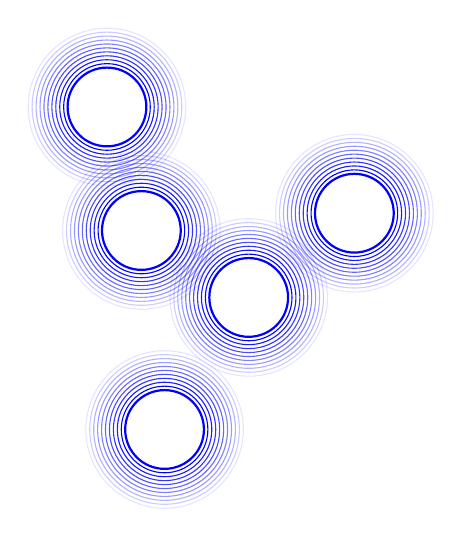
\begin{tikzpicture}[scale=0.5]
    % Dimensions de l'espace
    \pgfmathsetmacro{\width}{10}
    \pgfmathsetmacro{\height}{10}

    % Nombre de cercles
    \pgfmathsetmacro{\numcircles}{5}
    
    % Placer les cercles aléatoirement
    \foreach \i in {1,...,\numcircles} {
        \pgfmathsetmacro{\x}{rnd*\width}
        \pgfmathsetmacro{\y}{rnd*\height}
        
        % Dessiner la lueur bleue avec plusieurs cercles concentriques
        \foreach \j in {1,...,10} {
            \pgfmathsetmacro{\opacity}{0.1*(11-\j)}
            \draw[blue, opacity=\opacity] (\x,\y) circle (\j*0.1+1);
        }
        % Dessiner le cercle principal
        \draw[blue, thick] (\x,\y) circle (1);
    }
\end{tikzpicture}
\end{center}
We use the assumption of \citet{batchelor1972sedimentation} and assume linearity of the local scale equations. 
Therefore, we stipulate that $f_f^0(\textbf{x},t;\FF)$ can be subdivided by  
\begin{equation}
    f_f^0(\textbf{x},t;\FF)
    = 
    \sum_i
    f_{f\alpha}^0(\textbf{x},t;\FF)
\end{equation}
where $f_{fi}^0(\textbf{x},t;\FF)$ is the disturbance fields produce by the particle $i$ on $f_f^0$. 
This of course implies that $f_f^0 = 0$ in the absence of particle in the flow. 
Under this very restrictive hypothesis we can write, 
\begin{equation}
    \avg{\chi_ff_f^0}[\textbf{x},t]
    = 
    \sum_\alpha
    \avg{\chi_f f_{f\alpha}^0(\textbf{x},t;\FF)}
    = 
    \int_{\mathbb{R}^3} 
    \avg{
        \sum_\alpha
    \chi_f f_{f\alpha}^0(\textbf{x}_\alpha + \textbf{r},t;\FF) \delta(\textbf{x} - \textbf{x}_\alpha - \textbf{r})}d\textbf{r}
\end{equation}
assuming that \textbf{r} is relatively small compared to the macroscale we may write $\delta(\textbf{x} - \textbf{x}_\alpha - \textbf{r}) =\delta(\textbf{x} - \textbf{x}_\alpha) - \textbf{r}\cdot \grad\delta(\textbf{x} - \textbf{x}_\alpha)+ \ldots$
\begin{equation}
    \avg{\chi_ff_f^0}[\textbf{x},t]
    = 
    n_p(\textbf{x}) 
    \int_{\mathbb{R}^3} 
    f_{f\alpha}^1(\textbf{x}+ \textbf{r}| \textbf{x})
    d\textbf{r}
\end{equation}
with, 
\begin{equation*}
    f_{f\alpha}^1[\textbf{x}+ \textbf{r}| \textbf{x}]n_p(\textbf{x}) 
    = 
    \int{
    \sum_\alpha
    \chi_f f_{f\alpha}^0(\textbf{x}_\alpha + \textbf{r},t;\FF) \delta(\textbf{x} - \textbf{x}_\alpha)
    }d\PP
\end{equation*}
Not really satifying 

\subsection{The force traction term}

Let $f^1_f$ be an arbitrary \textit{single-particle} conditionally-averaged quantity. 
Notice that when $f^1_f$ is evaluated infinitely far from the particle we have the relation, 
\begin{equation*}
    \lim_{|\textbf{x} - \textbf{y}| \to \infty}  f^1_f [\textbf{y},t;\textbf{x},\textbf{c}] = f_f [\textbf{y},t]
\end{equation*}
Indeed, at large distance from a particle the \textit{single-particle} conditionally-averaged quantities are not influenced by the particles and therefore reduce to the classic averaged fields. 
Therefore, we define the distance field of a particle as $f^{1d}_f = f^1_f [\textbf{y},t;\textbf{x},\textbf{c}]  - f_f[\textbf{y},t]$ such that any disturbance field satisfy, 
\begin{equation*}
    \lim_{|\textbf{x} - \textbf{y}| \to \infty}  f^{1d}_f [\textbf{y},t;\textbf{x},\textbf{c}] = 0 
\end{equation*}
Using  $\bm\sigma_f^1 = \bm\sigma_f + \bm\sigma_f^{1d}$ these definitions we may write, 
\begin{equation}
    \pSavg{\bm\sigma_f^0\cdot\textbf{n}}[\textbf{x},t]
    =
    n_p(\textbf{x})
    \int_{\mathbb{R}^3}
    \int_{|\textbf{x}-\textbf{y}|=a}
    \bm\sigma_f
    \cdot \textbf{n}
    d\textbf{y}
    d\textbf{c}
    + n_p(\textbf{x})
    \int_{\mathbb{R}^3}
    \int_{|\textbf{x}-\textbf{y}|=a}
    \bm\sigma_f^{1d}
    \cdot \textbf{n}
    d\textbf{y}
    d\textbf{c}
    \label{eq:drag}
\end{equation}
Notice that $\bm\sigma_f$ is evaluated at $\textbf{y}$ therefore to get it out of the integration one can notice that $\bm\sigma_f(\textbf{y},t) = \bm\sigma_f(\textbf{x},t) + \textbf{r}\cdot \grad\bm\sigma_f(\textbf{x},t)+ \ldots$
where we have introduced $\textbf{r} = \textbf{y} - \textbf{x}$. 
Substituting the first two terms of this Taylor series into \ref{eq:drag} yields
\begin{equation}
    \pSavg{\bm\sigma_f^0\cdot\textbf{n}}[\textbf{x},t]
    =
    n_p v_p 
    \div\bm\sigma_f
    +
    n_p 
    \int_{|\textbf{x}-\textbf{y}|=a}
    \bm\sigma_f^{1d} \cdot \textbf{n}
    d\textbf{y}
    \label{eq:drag_final}
\end{equation}
Therefore, notice that drag force term has a component related to the mean fluid phase stress plus the contribution from the disturbance fields. 
Additionally, similar consideration can be made for the first two moments of the hydrodynamic force traction. 
This gives, 
\begin{align}
    \pSavg{\textbf{r}\bm\sigma_f^0\cdot\textbf{n}}[\textbf{x},t]
    =
    n_p v_p \bm\sigma_f
    +
    n_p 
    \int_{\mathbb{R}^3}
    \int_{|\textbf{x}-\textbf{y}|=a}
    \textbf{r}\bm\sigma_f^{1d} \cdot \textbf{n}
    d\textbf{y}
    d\textbf{c}
    \\
    \pSavg{\textbf{rr}\bm\sigma_f^0\cdot\textbf{n}}[\textbf{x},t]
    =
    n_pv_p  \frac{a^2}{5} 3 [(\div \bm\sigma_f)\bm\delta]^\text{sym}
    +
    n_p 
    \int_{\mathbb{R}^3}
    \int_{|\textbf{x}-\textbf{y}|=a}
    \textbf{rr}\bm\sigma_f^{1d} \cdot \textbf{n}
    d\textbf{y}
    d\textbf{c}
    \\
\end{align}
where the operator $[\ldots]^\text{sym}$ returns the symmetric part of the arguments.
Notice that the contribution from the mean stress in the second moment of the hydrodynamic force might become negligible for small $\phi_d$. 
In these expressions no hypothesis have been made. 


The fluid phase is a Newtonian thus, $\bm\sigma_f^0 = - p_f^0\bm\delta + 2\mu_f [\grad \textbf{u}_f^0 + (\grad \textbf{u}_f^0)^\dagger]$.
Therefore, the fluid phase stress averaged conditionally on the presence of a particle at \textbf{x} with the fluid phase at \textbf{y} might be written
\begin{align*}
    n_p \phi_f^1 \bm\sigma_f^{1d} = 
    n_p \phi_f^1 \bm\sigma_f^{1d} 
    - n_p \phi_f^1 \bm\sigma_f \\
    = - \phi_f^1 p_f^{1d}\bm\delta 
    + \mu_f \avg{\chi_f \delta_1 [\grad \textbf{u}_f^0 + (\grad \textbf{u}_f^0)^\dagger] }
    - \mu_f n_p \avg{\chi_f [\grad \textbf{u}_f^0 + (\grad \textbf{u}_f^0)^\dagger] }\\
    =- p_f^{1d}\bm\delta 
    + \mu_f \avg{(\delta_1 - n_p) [\grad \textbf{u}_f^0 + (\grad \textbf{u}_f^0)^\dagger] }
    - \mu_f \avg{\chi_d (\delta_1 - n_p) [\grad \textbf{u}_f^0 + (\grad \textbf{u}_f^0)^\dagger] }
\end{align*}
By noticing that both $\delta_1$ and $n_p$ commute with the derivatives and by noticing that  
\begin{equation*}
    \avg{(\delta_1 - n_p)  \textbf{u}^0}
    = 
    n_p \textbf{u}^{1d}
\end{equation*}
is the disturbance field of the bulk velocity conditionally on a particle present at $\textbf{y}$ we arrive at the relation 
\begin{align*}
    n_p \phi_f^1 \bm\sigma_f^{1d} = 
    - \phi_f^1 p_f^{1d} \bm\delta 
    + \mu_f n_p \left[\grad \textbf{u}^1 + (\grad \textbf{u}^1)^\dagger\right]
    - 2 \mu_f n_p \phi_d^1 \textbf{e}_d^{1d}
\end{align*}
where the second term is the contribution from the particle to the fluid phase stress, conditionally on the presence of the dispersed phase at \textbf{x} with a particle already present at \textbf{y}. 
Due to the simultaneous presence of $\phi_d$ and $n_p$ this term is negligible at first order in $\phi$. 

\subsection*{The consitional averaged Navier stokes equaiton}
As shown above $\bm\Sigma_f$ is function of the unknown of the problem so it is closed. 
The remaining term to compute is $\bm\Sigma_f^{1d}$ which is a function of $\textbf{u}_f^{1d}$ and $p_1^{1d}$. 
To obtain these fields one must solve the \textit{single-particle} conditionally-averaged equations for the disturbance fields  $\textbf{u}_f^{1d}$ and $p_1^{1d}$. 
Notice that we assume that the equation for  $\textbf{u}_f^{1d}$ and $p_1^{1d}$ follow the stokes hypothesis. 
However, in light of \ref{eq:dt_hybrid_rhou_f} the fields $\textbf{u}_f^{1}$ has no reason to follow the stokes limit hypothesis. 
For this reason we believe that (5.1) and (5.2) of \citet{zhang1997momentum} is not well posed. 

In all rigor to obtain the equations for the $\textbf{u}^{1d}$ one multiply the single-fluid formulation of the momentum \eqref{eq:dt_f} evaluated at \textbf{r} by $\sum_\alpha \delta(\textbf{x}-\textbf{x}_\alpha)$ and then average over all configuration,  and use $\textbf{u}^1 = \textbf{u}^{1d} - \textbf{u}$ to obtain an equation for the averaged fields only. 
This, yields
\begin{equation*}
    \pddt (n_p \rho^1 \textbf{u}^1)
    + \pddr  (
        n_p \rho^1 \textbf{u}^1  \textbf{u}^1 
        - n_p \bm\sigma^1
        )
    + \div (\rho^1 \textbf{u}^1 \textbf{u}_p^1  n_p )
    = 0. 
\end{equation*}
Where we have neglected covariance terms generated due to the product of the velocities.
At the zeroth order in $\div \textbf{u}^1[\textbf{r},t|\textbf{x}]$ ? $\div \textbf{u}_p[\textbf{x}]$ ? 

Then using the averaged Navier Stokes equations for $\textbf{u}_1$ one arrive to the stokes equations for $\textbf{u}_f^{1d}$, they read, 
\begin{align*}
    \div \textbf{u}_f^{1d} = 0 &&
    \div \bm\Sigma_f^{1d} = 0 
\end{align*}
Wit boundary condition 
\begin{align*}
    \textbf{u}_f^{1d}[\textbf{y},t|\textbf{x}] = 0 \text{  for  } |\textbf{r}| \to \infty\\
    \textbf{u}_f^{1d}\cdot \textbf{n}[\textbf{y},t|\textbf{x}] = (\textbf{v} - \textbf{u}_f)\cdot \textbf{n}[\textbf{y},t]\text{  on  } S_p
\end{align*}
According to the definition $\textbf{u}_f^{1d}$ the mean fluid velocity $\textbf{u}_f$ is evaluated at $\textbf{y}$, thus we might rewrite the second boundary condition as, 
\begin{align*}
    % \textbf{u}_f^{1d} = 0 \text{  for  } |\textbf{r}| \to \infty\\
    \textbf{u}_f^{1d} = \textbf{v} - \textbf{u}_f(\textbf{x},t)
    -\textbf{r}\cdot\grad\textbf{u}_f(\textbf{x},t)
    -\frac{1}{2}\textbf{rr}:\grad^2\textbf{u}_f(\textbf{x},t)
    \ldots
    \text{  on  } S_p
\end{align*}

These equations might be evaluated for two senarios

\subsubsection*{Computation of the fluid phase term}

For suspension of spherical particles in the dilute limit the fluid phase averaged fields may be simplyfied by noticing that $\phi_f^1[\textbf{x},t;\textbf{y},\textbf{c}] P_1[\textbf{y},\textbf{c},t] = P_1[\textbf{y},\textbf{c},t]$ when $|\textbf{x} - \textbf{y}| > a$. 
\begin{equation}
    \avg{\chi_f f_f^0}[\textbf{x},t]
    = 
    \int_{\mathbb{R}^3}
    \int_{\mathbb{R}^3}
    f_f^1 \phi_f^1[\textbf{x},t;\textbf{y},\textbf{c}] P_1[\textbf{y},\textbf{c},t]
    d\textbf{y} 
    d\textbf{c}
\end{equation}
where,
\begin{equation*}
    f_f^1 \phi_f^1[\textbf{x},t;\textbf{y},\textbf{c}] P_1[\textbf{y},\textbf{c},t]
    =     
    \int
    \frac{1}{N}
    \sum_\alpha \delta(\textbf{y}-\textbf{x}_\alpha)
     \delta(\textbf{c}-\textbf{u}_\alpha)
    \chi_f
    f^0_f[\textbf{x},t;\FF]
    d\PP.
\end{equation*}

\section{Singularity solution for spherical droplets}

\subsubsection*{A droplet in an arbitrary linear flows}

It is known that the velocity field around and inside a droplet immersed in an arbitrary linear flow is written,
\begin{equation}
    \textbf{u}_f^1(\textbf{r})
    = 
    \mathcal{U}_f\cdot \textbf{u}_{fp}
    + \mathcal{E}_f: \textbf{E}_{f}
\end{equation}
\begin{equation}
    \textbf{u}_d^1(\textbf{r})
    = 
    \mathcal{U}_d\cdot \textbf{u}_{fp}
    + \mathcal{E}_d: \textbf{E}_{f}
\end{equation}
where the second and third order tensor $\mathcal{U}$ and $\mathcal{E}$ read as, 
\begin{align}
    \mathcal{U}_{ik,f} = 
    \frac{1}{4}\left(\frac{3\lambda + 2}{\lambda +1}\right)
    \left(\frac{\delta_{ik}}{r} + \frac{r_ir_k}{r^3}\right) 
    + 
    \frac{1}{4}\left(\frac{\lambda}{\lambda +1}\right)
    \left(\frac{\delta_{ik}}{r^3} - \frac{3r_ir_k}{r^5}\right)  \\
    \mathcal{E}_{ijk,f}
    =
    %  \bm\delta\textbf{r}
    -\frac{\lambda}{(\lambda + 1)r^5} \bm\delta\textbf{r}
    -\left(\frac{5\lambda +2}{2(\lambda +1 )r^5} - \frac{5\lambda}{2(\lambda+1)r^7}\right) \textbf{rrr}
\end{align}
\begin{align}
    \mathcal{U}_{ik,d} = 
    \frac{1}{2}\left(\frac{2\lambda +3}{\lambda +1}\right)\bm\delta
    -\frac{1}{2} (2r^2 \bm\delta - \textbf{rr})
    \left(\frac{1}{\lambda +1}\right)\\
    \mathcal{E}_{ijk,d}
    =
    \frac{5r^2 -3}{2(\lambda +1)} \textbf{r}\bm\delta
    - \frac{1}{\lambda+1}\textbf{rrr}
\end{align}
where the \textbf{r} are made dimensionless with the particle radius. 
When evaluating these expressions at the particle surface yields, 
\begin{align}
    \mathcal{U}_{ik} = 
    % \frac{1}{4}\left(\frac{3\lambda + 2}{\lambda +1}\right)
    % \left(\delta_{ik} + r_ir_k\right) 
    % + 
    % \frac{1}{4}\left(\frac{\lambda}{\lambda +1}\right)
    % \left(\delta_{ik} - 3r_ir_k\right)  \\
    \frac{1}{2}\left(\frac{2\lambda + 1}{\lambda +1}\right)
    \delta_{ik} 
    + 
    \frac{1}{2}\left(\frac{1}{\lambda +1}\right)
    r_ir_k  \\
    \mathcal{E}_{ijk}
    = 
    % \left[1-
    \frac{\lambda}{(\lambda + 1)}
    % \right]
    \bm\delta\textbf{r}
    -\left(\frac{2}{2(\lambda +1 )} \right) \textbf{rrr}
\end{align}
Remember that these was the expression of the disturbance flow we therefore must add the velocity of the fluid plus its gradient. 
Thus in the reference attached to the particle we have, 
\begin{equation*}
    \textbf{w}_d^0 
    = \left(\frac{\lambda + \frac{1}{2}}{\lambda +1} - 1\right)
    \textbf{u}_{pf} 
    + 
    \frac{1}{2}\left(\frac{1}{\lambda +1}\right)
    \textbf{rr} \cdot \textbf{u}_{pf} 
    + \left[1-\frac{\lambda}{(\lambda + 1)}\right]\textbf{E}_f\cdot\textbf{r}
    -\left(\frac{2}{2(\lambda +1 )} \right) \textbf{r} \textbf{E}_f:\textbf{rr}
\end{equation*}


\subsection*{A translating droplets}
\label{ap:Translating_sphere}

\tb{Consider using the famous reciprocal theorem  ?  ? ? ? }

\tb{This is usefull to derive the faxen contribution }

\tb{this is not usefull to derive the spetical contribution . . .}


In this appendix we expose the velocity fields solution for the stokes flow past a spherical drop. 
In a second step, we compute the form of the moment of momentum closure mentioned in \ref{sec:Lagrangian} in terms of the fluid properties and the drop fluid relative velocity.

We consider a drop of radius $a$ translating with the velocity $\textbf{u}_\alpha$ in a stokes flow with undisturbed velocity $\textbf{u}_1$.
The relative velocity between the droplet and the fluid is defined as $\textbf{u}_{\alpha 1}= \textbf{u}_\alpha - \textbf{u}_1(\textbf{x}_\alpha)$ where $\textbf{u}_1(\textbf{x}_\alpha)$ is the undisturbed averaged fluid velocity at the position $\textbf{x}_\alpha$. 
In these conditions, the local fluid phase velocity $\textbf{u}_1^0$, the local particle interior velocity $\textbf{u}_2^1$ and the local stress fields $\bm\sigma_2^0$ within the particle phase, might be written as\citet{pozrikidis1992boundary}\footnote{The solution of this problem is derived in the above cited book p .207.  However, the author made a slight mistakes on the constant $\textbf{c}$ which we corrected here. }, 
\begin{align*}
    u_{1,i}^0
    = \left(\frac{\delta_{ik}}{r} + \frac{r_ir_k}{r^3}\right)  g_k
    + \left(-\frac{\delta_{ik}}{r^3} + \frac{3r_ir_k}{r^5}\right)  d_k\\
    u_{2,i}^0
    = c_i
    + \left(2 r^2 \delta_{ik} - r_ir_k\right) e_k\\
    % e_{2,ik}^0
    % = \mu(
    %     3 \delta_{ij} r_k 
    %     + 3 \delta_{kj} r_i
    %     -2 r_j \delta_{ki}
    % )e_j 
    \sigma_{2,ik}^0
    = \mu 3(
        - 4 \delta_{ik} r_j
        + \delta_{ij} r_k
        + r_i \delta_{kj}
    )e_j 
\end{align*}
with, 
\begin{align*}
    &\textbf{g} = a\frac{1}{4}\left(\frac{3\lambda + 2}{\lambda +1}\right) \textbf{u}_{\alpha 1},
    &\textbf{d} = -a^3\frac{1}{4}\left(\frac{\lambda}{\lambda +1}\right) \textbf{u}_{\alpha 1},\\
    &\textbf{c} = \frac{1}{2}\left(\frac{2\lambda + 3}{\lambda +1}\right) \textbf{u}_{\alpha 1},
    &\textbf{e} = -\frac{1}{a^2}\frac{1}{2}\left(\frac{1}{\lambda +1}\right)  \textbf{u}_{\alpha 1}.\\
\end{align*}

Now that we have an explicit solution for the internal flow and stress one can compute the terms appearing in the energy and moment of momentum balance equations. 
The integral involving the particle internal motion in the equation exposed in \ref{sec:Lagrangian} are evaluated exhaustively and yield, 
\begin{equation*}
    \intO{\rho_2(\textbf{w}_2^0)_i (\textbf{w}_2^0)_j}
    = \frac{m_\alpha}{140 (\lambda +1)^2}
    (7 (\textbf{u}_{\alpha 1})_i(\textbf{u}_{\alpha 1})_j + (\textbf{u}_{\alpha 1}\cdot \textbf{u}_{\alpha 1})\delta_{ij})
\end{equation*} 
\begin{equation*}
    \intO{\rho_2(\textbf{w}_2^0)_k (\textbf{w}_2^0)_k}
    = \frac{m_\alpha}{14 (\lambda +1)^2}
     (\textbf{u}_{\alpha 1})_k(\textbf{u}_{\alpha 1})_k
\end{equation*} 
\begin{equation*}
    \intO{\rho_2(\textbf{w}_2^0)_i (\textbf{w}_2^0)_j}^\text{dev}
    = \frac{m_\alpha}{20 (\lambda +1)^2}
    ((\textbf{u}_{\alpha 1})_i(\textbf{u}_{\alpha 1})_j + (\textbf{u}_{\alpha 1}\cdot \textbf{u}_{\alpha 1})\delta_{ij})
\end{equation*} 
\begin{equation*}
    \intO{\bm\sigma_2^0}
    = 0 
\end{equation*}
\begin{equation*}
    \intO{\bm{\sigma}_2^0:\grad \textbf{u}_2^0}
    = 2\mu_2 \intO{\textbf{e}_2^0: \textbf{e}_2^0 }
    = 
    \frac{6 \mu_2 v_p}{a^2(1+\lambda)^2}
    (\textbf{u}_{\alpha 1}\cdot \textbf{u}_{\alpha 1})
\end{equation*}
\begin{align*}
    \intO{\textbf{r}\textbf{u}_2^0}
    = 0 
\end{align*}
\begin{equation*}
    \intS{\bm\sigma_1^0\cdot \textbf{n}_2}
    = - \frac{3v_\alpha\mu_1}{2 a^2} 
    \left(\frac{3\lambda+2}{\lambda+1}\right) 
    \textbf{u}_{\alpha 1}
\end{equation*}
\begin{equation*}
    \intS{\textbf{r}\bm\sigma_2^0\cdot \textbf{n}_2}
    = 0 
\end{equation*}
\begin{equation*}
    \intS{(\bm\sigma_2^0\cdot \textbf{n}_2)_i r_kr_l}
    = \frac{3\mu_1\phi_2}{10}\left(\frac{5\lambda+2}{\lambda+1}\right)u_{1 \alpha,i}\delta_{kl}
    + \frac{3\mu_1\phi_2}{5}\left(\frac{1}{\lambda+1}\right)(u_{1 \alpha,k}\delta_{il}+u_{1 \alpha,l}\delta_{ki})
\end{equation*}
\begin{equation*}
    \intO{\mu(\textbf{e}_2^0)_{ik} r_l} =
    \frac{\phi_2\mu_1}{10}\left(\frac{1}{\lambda+1}\right)
    \left(
        2\delta_{ik}u_{1 \alpha , l}
        -3\delta_{kl}u_{1 \alpha , i}
        -3\delta_{il}u_{1 \alpha , k}
    \right)
\end{equation*}
\begin{equation*}
    \int_{r>a} \mu_f \bm\sigma^0_f:\grad \textbf{u}_f  d\textbf{r}
    = 
\end{equation*}
We can notice that now all these quantities are determined by the relative velocity.  
While the hill vortex is a solution valid in potential and stokes flow, the solution for the exterior flow is limited to stoke flow. 
Consequently, the zero, first and second moment of surface force are limited to stokes flow. 

\subsection{A droplet in shear flow}

We consider an infinite linear flow $\textbf{u}^\infty = \bm\Gamma\cdot \textbf{r} =(\bm\Omega + \textbf{E})\cdot \textbf{r} $ such that the undisturbed flow around the sphere is $\textbf{u}^\infty = \bm\Gamma\cdot\textbf{r}$.
The disturbance flow in this case might be determined following the method outlined in \citep{leal2007advanced}, we obtain  :
\begin{align*}
    \textbf{u}^0_1
    = \bm\Gamma\cdot\textbf{r}
    -\frac{\lambda}{(\lambda + 1)r^5} \textbf{E}\cdot\textbf{r}
    - \left(\frac{5\lambda +2}{2(\lambda +1 )r^5} - \frac{5\lambda}{2(\lambda+1)r^7}\right) \textbf{r}(\textbf{E}:\textbf{rr})\\
    p_1^0 
    = -\frac{(5\lambda+2)}{(\lambda+1)r^5}\textbf{E}:\textbf{rr}\\
% \end{align*}
% \begin{align*}
    \textbf{u}^0_2
    = \bm\Omega\cdot\textbf{r}
    + \frac{5r^2- 3}{2(\lambda + 1)} 
    \textbf{E}\cdot\textbf{r}
    -\frac{1}{\lambda+1} \textbf{r}(\textbf{E}:\textbf{rr})\\
    p_2^0 
    = \frac{21\lambda}{2(\lambda+1)}
    \textbf{E}:\textbf{rr}
\end{align*}

With that we are able to compute the following integrals,
\begin{equation*}
    \intO{\rho_2(\textbf{w}_2^0)_i (\textbf{w}_2^0)_j}
    = \frac{4\pi}{15}\bm\Omega\cdot\bm\Omega
    + \frac{4\pi}{945(\lambda+1)^2}
    (2\textbf{E}:\textbf{EI} + 15 \textbf{E}\cdot \textbf{E})
\end{equation*}
\begin{equation*}
    \intO{\rho_2(\textbf{w}_2^0)_k (\textbf{w}_2^0)_k}
    = \frac{4\pi}{15}\bm\Omega:\bm\Omega
    + \frac{4\pi}{45(\lambda+1)^2}
    \textbf{E}:\textbf{E} 
\end{equation*} 
\begin{equation*}
    \intO{\bm\sigma_2^0}
    = \frac{8\pi}{5(\lambda+1)}
    \textbf{E}
\end{equation*}
\begin{equation*}
    \intO{\textbf{e}_2^0}
    = \frac{4\pi}{5(\lambda+1)}
    \textbf{E}
\end{equation*}
\begin{equation*}
    \intO{\bm{\sigma}_2^0:\grad \textbf{u}_2^0}
    = 2\mu_2 \intO{\textbf{e}_2^0: \textbf{e}_2^0 }
    = 
    \frac{4\pi}{(\lambda+1)^2}\textbf{E}:\textbf{E}
\end{equation*}
\begin{align*}
    \intO{\textbf{r}\textbf{u}_2^0}
    = 0 
\end{align*}
\begin{equation*}
    \intS{\bm\sigma_1^0\cdot \textbf{n}_2}
    = 0
\end{equation*}
\begin{equation*}
    \intS{\textbf{r}\bm\sigma_1^0\cdot \textbf{n}_2}
    = \frac{4\pi}{5}\frac{5\lambda+2}{\lambda+1}\textbf{E} 
\end{equation*}
\begin{equation*}
    \intS{(\bm\sigma_2^0\cdot \textbf{n}_2)_i r_kr_l}
    = 0
\end{equation*}
\begin{equation*}
    \intO{\mu(\textbf{e}_2^0)_{ik} r_l} =
    0
\end{equation*}